%%
%% This is file `thesis-ex.tex',
%% generated with the docstrip utility.
%%
%% The original source files were:
%%
%% uiucthesis2009.dtx  (with options: `example')
%% 
\def\fileversion{v2.25a} \def\filedate{2009/10/10}
%% Package and Class "uiucthesis2009" for use with LaTeX2e.
\documentclass[edeposit,fullpage]{uiucthesis2009}
\usepackage{amsfonts}
\usepackage{amssymb}
\usepackage{amsmath}
\usepackage{hyperref}
\usepackage{graphicx}% Include figure files
\usepackage{epstopdf}
\usepackage{subfig}
\usepackage{makeidx}
\usepackage{appendix}
\input{../newcommand}
\begin{document}

\title{BCS-BEC Crossover with Feshbach Resonance for Three-Hyperfine-Species Model}
\author{Guojun zhu}
\department{Physics}
\schools{B.S., University of Science and Technology of China, 2001\\
         M.S, University of Illinois at Urbana-Champaign, 2003}
\phdthesis
\advisor{Anthony Leggett}
\degreeyear{2011}
\committee{Professor Gordon Baym\\Professor Brian DeMarco\\Professor Scott Willenbrock\\Professor Anthony Leggett}
\maketitle

\frontmatter

%% Create an abstract that can also be used for the ProQuest abstract.
%% Note that ProQuest truncates their abstracts at 350 words.
\begin{abstract}
This is a comprehensive study of caffeine consumption by graduate
students at the University of Illinois who are in the very final
stages of completing their doctoral degrees. A study group of six
hundred doctoral students\ldots.
\end{abstract}

%% Create a dedication in italics with no heading, centered vertically
%% on the page.
\begin{dedication}
To Jie, Ethan and Chloe
\end{dedication}

%% Create an Acknowledgements page, many departments require you to
%% include funding support in this.
\chapter*{Acknowledgments}
This thesis would not be possible without the guidance and patience from my advisor, Prof. Anthony J. Leggett.  I would like to thank Prof. Monique Combescot from Paris especially for her help, kindness and lots of invaluable advise.  Also, I would like to thank Dr. Wei-Cheng Lee, Dr. Shizhong Zhang, Dr. Parag Ghosh for their many discussion and suggestion.  Finally I would thank my wife and my family for constant support and affection all the time.  

%% The thesis format requires the Table of Contents to come
%% before any other major sections, all of these sections after
%% the Table of Contents must be listed therein (i.e., use \chapter,
%% not \chapter*).  Common sections to have between the Table of
%% Contents and the main text are:
%%
%% List of Tables
%% List of Figures
%% List Symbols and/or Abbreviations
%% etc.

\tableofcontents
\listoftables
\listoffigures

%% Create a List of Abbreviations. The left column
%% is 1 inch wide and left-justified
\chapter{List of Abbreviations}

\begin{symbollist*}
\item[w.f.] wave function.
\end{symbollist*}

%% Create a List of Symbols. The left column
%% is 0.7 inch wide and centered
\chapter{List of Symbols}

\begin{symbollist}[0.7in]
\item[$\psi$] wave function.
\end{symbollist}

\mainmatter
% !TeX root =thesis.tex

\chapter{Introduction}
Feshbach resonance is widely used in the ultracold alkali gas experiments as an indirect way to tune interaction strength.  This unique ability gives physicist the opportunity to study the evolution of many-body system under change of interaction strength, which connects different systems originally under different frameworks.  Particularly for the fermion system, there was long theoretically work about uniform treatment over BEC and BCS \cite{Eagle,LeggettCrossover,Nozieres,RanderiaBEC}, and Feshbach resonance within the ultracold alkali gas provide the perfect grounds to verify it.  Within the lowest order, the theory works remarkably well, the experiments fit it qualitatively.  

Here we actually try to look into the idiosyncratic of the Feshbach resonance as comparing to a real ``Simple'' knob on the interaction strength.  Within the two-body description of Feshbach resonance, there is a parameter $\delta_c$ describing how close to resonance is necessary to have substantial weight in close-channel.  Combining this with a many-body problem, a simple question is how this energy scale compares to a typical many-body energy scale, Fermi energy.  If Fermi energy is much smaller comparing to $\delta_c$, (\emph{broad resonance}), close-channel can be safely ignored at many-body level and the problem can be well-described as a two-species fermion system with tunable interaction.  On the contrary, when Fermi energy is larger than or comparable to $\delta_c$, close-channel cannot be ignored in many-body level.  Nevertheless, another important thing in the problem is that we are dealing with a Feshbach resonance with a relatively tight-bound close-channel state, which is much smaller comparing to other many-body scale.  Therefore, we are never dealing with a true three(four)-species Fermion system, which probably requires quite different techniques to solve.

To complicate the problem even further, the real experiments system often has one common species.  Pauli exclusion prevents the same species occupy both channels.  This effect has no counter-part in two-body problem, and will be one of the central problems in this study. 

Roughly speaking, many-body nature brings two effects.  The first one closely associates with Fermi energy.  At low temperature, most fermions are inactive and only fermions close to fermi surface can participate, therefore, energy often needs to be measured from Fermi sea instead of zero as in two-body situation.  It always relates to Fermi Energy $E_F$.  This effect has been extensively studied in \cite{GurarieNarrow}.

The second effect is unique for the three-species problem.  Phase spaces of two channels are overlapped because of the Pauli exclusion from the common species. This effect is controlled by overlapping of states in two channels. We can estimate it roughly.  In the close-channel, bound-state is relatively small, and binding energy $E_b$ is close to absolute energy difference between two channels, $\eta$.  On the other hand, fermions in open-channel occupies the lowest states in the momentum space and therefore spread out in space.  The typical energy scale would be $E_F$.  Therefore a ratio $E_F/\eta$ would control such effect. 

Alternatively, we can make a rough estimation on simple double-fermion molecule gas.  If we assume the molecule size is $r_{c}$ and the total number is $N$.  If assume further that the bound-state is close-to-threshold.  We will have wave function $A/(k^{2}+\kappa^{2})$, where $\hbar^{2}\kappa^{2}/2m=E_{b}$, (see Appendix \ref{sec:pathInt2:short-range}) and $\sum_{k=0}^{1/r_{c}}\psi^{2}\sim{}N$, now if we considering only particles within range $E_{F}\ll\kappa$, the total particle in it is roughly $N\cdot(k_{F}r_{c})$.  this number can be much smaller than $N$. Put this into the perspective of two-channel problem, the low-momentum is still dominated by open-channel component even when total weight of close-channel is comparable or higher than it of open-channel because close-channel is mostly in high-momentum state.    

\section{Two-body Feshbach resonance problem}
Here we will briefly review the Feshbach resonance in two-body setup, we will mostly follow treatment in \cite{Leggett}.
\section{Single-channel BEC-BCS crossover}
Here we will briefly review the BEC-BCS crossover in single channel.   Here the interaction strength is tuned along the crossover region.  This applies to the broad-resonance, where the close-channel weight is negligible and serves only to modify the effective strength in open-channel.  We will mostly follow treatment in \cite{Leggett}.
\chapter{Path-Integral approach}
\section{Path integral for one channels}
% !TeX root =thesis.tex
%\subsection{Path integral approach for single channel\label{sec:pathInt}}
\label{sec:pathInt}
They have studied this problem with a path integral approach which is proved to be a  nice tool for the problem due to its flexibility and readiness to be   extended for the higher order fluctuations.  In the next two chapters, this method will be adapted  further for the two-channel model. 

We start with an attractive $\delta$-potential in the coordinate space.  This potential is not equivalent to the  reduced pairing potential used in the original BCS work.  The reduced pairing potential only couples  particles of the opposite momentum and does not support simple form of Hubbard-Stratonovich transformation, which is essential to solve the problem in the path integral formulation. 

  The Hamiltonian with the chemical potential of the system can be written as   
\begin{equation}
\hat{H}-\mu\hat{N}=\sum_{\sigma}\int{d^{d}\vr}c^{\dagger}_{\sigma}(\vr)\br{-\nth{2m}\nabla^{2}-\mu}c^{}_{\sigma}(\vr)-g\int{d^{d}\vr}c^{\dagger}_{\uparrow}(\vr)c^{\dagger}_{\downarrow}(\vr)c^{}_{\downarrow}(\vr)c^{}_{\uparrow}(\vr)
\end{equation}
Introducing the quantum partition function $\mathcal{Z}=\int{\bigD(\bar\psi,\psi)\exp\br{-S[\bar\psi,\psi]}}$, where $\bigD(\bar\psi,\psi)$ denotes the functional integral over all possible wave function $\psi$ and $\bar\psi$, and the action $S[\bar\psi,\psi]$ can be written down from the Hamiltonian
\begin{equation}\label{eq:pathInt2:actionPsi}
S[\bar\psi,\psi]=\int^{\beta}_{0}d\tau\int{d^{d}\vr}\mbr{\sum_{\sigma}\bar\psi_{\sigma}(\vr,\tau)\br{\partial_{\tau}-\nth{2m}\nabla^{2}-\mu}\psi_{\sigma}(\vr,\tau)-g\bar\psi_{\uparrow}(\vr,\tau)\bar\psi_{\downarrow}(\vr,\tau)\psi^{}_{\downarrow}(\vr,\tau)\psi^{}_{\uparrow}(\vr,\tau)}
\end{equation}
The fermion fields $\psi_{\sigma}$ and $\bar\psi_{\sigma}$ being two independent Grassmann variables, notice that  they are not complex conjugate to each other as in the usual operator language because  complex conjugate is not a well-defined concept for Grassmann variables. 

This system can be solved with Hubbard-Stratonovich transformation.   Introduce an auxiliary field (functional variable) $\Delta(\vr,\tau)$ coupled with a pair $\psi_{\uparrow}(\vr,\tau)\psi_{\downarrow}(\vr,\tau)$. %Here we follow the normal notation from path integral, $r$ is four tempo-space coordinator.  
We write down first the Gaussian integral of $\Delta$
\begin{equation}
1=\int{\bigD(\bar\Delta,\Delta)}\exp\br{-\nth{g}\int{d\tau{d}^{d}r}\bar\Delta\Delta}
\end{equation}
Note that we absorb the extra constant of integration into the measure of $\bigD(\bar\Delta,\Delta)$.
And with a shift of $\Delta(\vr,\tau)\rightarrow\Delta(\vr,\tau)-g\psi_{\uparrow}(\vr,\tau)\psi_{\downarrow}(\vr,\tau))$, we have 
\footnote{$\int{\bigD(\bar\Delta,\Delta)}\cdot1$ is only a constant factor on partition function $\mathcal{Z}$ and has no effect on real physical quantity; therefore, we can take it as 1. (This is equivalent to  divide the $\mathcal{Z}$ by a constant)}
\begin{equation}\label{eq:pathInt:expHS}
\exp\br{g\int{d\tau{}d^{d}r}\bar{\psi}_{\uparrow}\bar\psi_{\downarrow}\psi_{\downarrow}\psi_{\uparrow}}=
\int{\bigD(\bar\Delta,\Delta)}\exp\bbr{-\int{d\tau{d^{d}r}}\mbr{\nth{g}{\bar\Delta}{\Delta}-\br{\bar\Delta\psi_{\downarrow}\psi_{\uparrow}+\Delta\bar\psi_{\uparrow}\bar\psi_{\downarrow}}}}
\end{equation}
Note that  $\Delta(\vr,\tau)$ (or $\bar\Delta(\vr,\tau)$) comes from  Grassmann fields $\psi(\vr,\tau)$ (or $\bar\psi(\vr,\tau)$). Therefore, they are not related to each other as complex conjugate either.  Nevertheless, at the mean field level or only at the phase fluctuation around the mean field values, $\Delta$  and $\bar\Delta$ are indeed complex conjugate.  Consequently, we will just take $\Delta$  as normal bosonic field in the following and often simply treat $\bar\Delta$ as $\Delta$'s complex conjugate in the following. Now the interaction term can be replaced.
\begin{align*}
\mathcal{Z}=&\int{}\bigD(\bar\psi,\psi)\int{\bigD(\bar\Delta,\Delta)}\\
&\;\exp\bbr{-\int{d\tau{d^{d}r}}\mbr{\sum_{\sigma}\bar\psi_{\sigma}\br{\partial_{\tau}-\nth{2m}\nabla^{2}-\mu}\psi_{\sigma}+\nth{g}{\bar\Delta}{\Delta}-\br{\bar\Delta\psi_{\downarrow}\psi_{\uparrow}+\Delta\bar\psi_{\uparrow}\bar\psi_{\downarrow}}}}
\end{align*}
At the expense of introducing an auxiliary field ($\Delta$) which has contact-type coupling to the original field $\psi$, we eliminate the four-field interaction term formally.  $\Delta$ field is like a \emph{local potential} for $\psi$, although this \emph{local potential} has to be calculated from the original field self-consistently.  Nevertheless, $\Delta$ couples to a pair of fermionic field $\psi$, and thus it extracts a special degree of freedom from the $\psi$ field.  When properly selected, this degree of freedom is highly non-trivial and has macroscopic importance, which serves as ``order parameter'' for the system.  The above formula for partition function is bilinear to $\psi$, and we can rewrite it into a nicer form in Nambu spinor representation
\begin{equation}
\bar\Psi=\begin{pmatrix}\bar{\psi}_{\uparrow}&\psi_{\downarrow}\end{pmatrix}\text{,  }\qquad
\Psi=\begin{pmatrix}{\psi}_{\uparrow}\\\bar\psi_{\downarrow}\end{pmatrix}
\end{equation}
\begin{equation}\label{eq:pathInt:ZDeltaPhi}
\mathcal{Z}=\int{\bigD(\bar\Psi,\Psi)}\int{\bigD(\bar\Delta,\Delta)}\exp
	\bbr{-\int{d\tau{d^{d}r}}\mbr{\nth{g}{\bar\Delta}{\Delta}-\bar\Psi \nG\Psi}}
\end{equation}
where 
\begin{equation}\label{eq:pathInt:nG}
\nG=\begin{pmatrix}
[\hat{G}_{0}^{(p)}]^{-1}&\Delta\\\bar\Delta&[\hat{G}_{0}^{(h)}]^{-1}
\end{pmatrix}
\end{equation}
is known as the Gor'kov Green function. $[\hat{G}_{0}^{(p)}]^{-1}=-\partial_{\tau}+\nth{2m}\nabla^{2}+\mu$, and $[\hat{G}_{0}^{(h)}]^{-1}=-\partial_{\tau}-\nth{2m}\nabla^{2}-\mu$ represent the non-interacting Green functions of the particle and the hole respectively. 

Before going further, we would like to discuss one confusing point about the possible one-or-two indices for quantities such as ${G}$ or $\Delta$ in Eq. \ref{eq:pathInt:nG}.  As a matrix, such a quantity has two indices $(x,x')$ or $(p,p')$, which have no ambiguity in usage. On the other hand, there are often ambiguity when only one index $x$ or $p$ is used. In some cases, the one index means the relative value of the two indices. For example, an  interaction, $U(\vr_{1},\vr_{2})$, normally only depends on the relative coordinate, $\vr=\vr_{1}-\vr_{2}$. So $U(\vr)$ means $U(\vr_{0}+\vr,\vr_{0})$.  In other cases, especially common in the current thesis, the one index stands for its repetition.  In this case, the difference is always zero. For example, the free Green's function, $G_{0}(p)$ stands for $G_{0}(p,p')\delta({p-p'})$.  Similarly,  the order parameter, $\Delta(x)$, only couples to $\bar\psi(x)\bar\psi(x)$ (Eq. \ref{eq:pathInt:expHS}).  When used in the matrix context (Eq. \ref{eq:pathInt:nG}), it means $\Delta(x)\delta(x-x')$. Interestingly, its Fourier transformation in momentum space does not have the same properties.  In fact, it means $\Delta(p,p')=\Delta(p'-p)$.

Now action in Eq. \ref{eq:pathInt:ZDeltaPhi} is bilinear to $\Psi$; so it can be integrated out formally and the partition function then only depends on the  field $\Delta$.  
\begin{equation}\label{eq:pathInt:DeltaPF}
\mathcal{Z}=\int{\bigD(\bar\Delta,\Delta)}\exp
	\bbr{-\mbr{\br{\int{d\tau{d^{d}r}}\nth{g}{\bar\Delta\Delta}}-\ln\det\nG}}
\end{equation}
And the action becomes
\begin{equation}\label{eq:pathInt:DeltaAction}
S[\bar\Delta,\Delta]=
	{\mbr{\br{\int{d\tau{d^{d}r}}\nth{g}{\bar\Delta\Delta}}-\ln\det\nG}}
\end{equation}
Note that the determinant in $\ln\det\nG$ runs through both the normal coordinate space and $2\times2$ Nambu spinor space.  The above formulas are exactly equivalent to the original partition function (action) in the fermion field $\psi$ (Eq. \ref{eq:pathInt2:actionPsi}). It looks nice and compact. Nevertheless, $\ln\det\nG$ term is highly non-trivial and contains all the many-body physics.

\section{Mean field results\label{sec:pathInt:meanfield}}
The saddle point equation of Eq. (\ref{eq:pathInt:DeltaPF}) gives the mean-field result of the system.  First we need to find the derivative of $\ln\det\nG$.  We notice the identity
\begin{equation}
\ln\det\hat{A}=\tr\ln\hat{A}
\end{equation}
and differential rule of the function ``$\tr\ln$''
\begin{equation}\label{eq:pathInt:diffTr}
\frac{\delta}{\delta\phi_q}\tr\ln(\nG)=\tr(\hat{\mathcal{G}}\frac{\delta}{\delta\phi_q}\nG)
\end{equation}
Using the above relations, we can write the saddle equation of Eq. (\ref{eq:pathInt:DeltaPF}) (differential with respect to $\Delta$) as
\begin{equation}
\nth{g}\bar{\Delta}(\vr,\tau)-\tr\mbr{\hat{\mathcal{G}}(\vr,\tau,\vr,\tau)\begin{pmatrix}0&1\\0&0\end{pmatrix}}=0
\end{equation}
Here this matrix is in the Nambu Spinor space.  At the  mean field level, we seek a tempo-spacial homogeneous solution of $\Delta(x)=\Delta_{0}$.  At this level,  $\Delta(p)$ becomes a $\delta$-function in the frequency-momentum space, and has non-zero elements only for two fermions with the same momentum.  (Please See the discussion in the previous section about one vs. two indices. This is not generally true, as we show it when discussing collective modes in sec. \ref{sec:collective1})
We can find the Gor'kov Green function from Eq. (\ref{eq:pathInt:nG}) in momentum space at the mean-field level
\begin{equation}\label{eq:pathInt:G0}
G_{0\;p,p'}=\nth{(i\omega_n)^2-E_\vp^2}
\begin{pmatrix}
	i\omega_n+\xi_\vp&\;&-\Delta_0\\
	-\bar{\Delta}_0&\;&i\omega_n-\xi_\vp
\end{pmatrix}
\delta_{p=p'}
\equiv{}G_{0}(p)\delta_{p=p'}
\end{equation}
Here $p$ is the frequency-momentum, $p=(\omega_{n},\vp)$, and $\omega_n$ is the Matsubara frequency of Fermions.  $\xi_{\vk}=\epsilon_{\vk}-\mu$, $\epsilon_{\vk}=\vk^{2}/2m$,  $E_\vp=\sqrt{\xi_\vp^2+\abs{\Delta_0}^2}$.  And the saddle point equation can be rewritten as 
\begin{equation}
\nth{g}\bar{\Delta}_0=\frac{T}{\mathcal{V}_{0}}\sum_{\vp,n}\frac{\bar\Delta_0}{\omega_n^2+E_\vp^2}
\end{equation}
Here $T$ is the temperature, and $\mathcal{V}_{0}$ is the volume in $d$-dimension.  The summation of Matsubara frequency  can be evaluated\footnote{\label{foot:intro:sum}The summation of the Matsubara frequency of a function $h(i\omega_{n})$ is carried out by the normal trick.  We  multiply $h(z)$ with the Fermi distribution function $n_{F}(z)$,  the summation is the sum of residuals at the imaginary axis of $n_{F}(z)$.  The contour can be deform into a contour over the rest of singular points of $h(z)$. We just need to find the residuals of the total function $h(z)n_{F}(z)$ over those singular points to find the Matsubara summation.   However, due to zero temperature, the  $n_{F}(z)$ is only nonzero at the negative singular points of $h(z)$, $-E_{\vk}$ in this case.  (The other singular point $E_{\vk}$ gives $n_{F}(E_{\vk})=0$ for zero temperature.)}  and we find 
\begin{equation}
\nth{g}=\nth{\mathcal{V}_{0}}\sum_{\vp}\frac{1-2n_f(E_p)}{2E_p}=\nth{\mathcal{V}_{0}}\sum_{\vp}\frac{\tanh{(E_p/2T)}}{2E_p}
\label{eq:pathInt:gap}
\end{equation}
where $n_f(\epsilon)$ is the fermi distribution function.  This is exactly the famous gap equation obtained from other methods as well.  On the other hand, $\nG$ in Eq. (\ref{eq:pathInt:nG})  is the inverse of the  fermion-fermion correlation of $\Psi$.  In the mean field, $G_{0}$ as Eq. (\ref{eq:pathInt:G0}) can be diagonalized in the momentum space with a canonical (Bogoliubov) transformation.  We can make an analytic continuation of $i\omega_{n}\rightarrow\omega+0^{+}$.  Eq. (\ref{eq:pathInt:G0})  then has poles ($\pm{}E_{p}$) where  $\omega^2-E_\vp^2=0$,  which determine  the spectrum of fermionic excitation.  Indeed, in the BCS-like states ($\mu>0$), the spectrum is gapped at $\Delta$; while in the BEC-like states ($\mu<0$), the fermionic excitation starts from the molecule binding energy $\sqrt{\mu^{2}+\Delta^{2}}\approx\abs{\mu}$.

 The summation in Eq. (\ref{eq:pathInt:gap})  does not converges  in 3D because the summand does not decreases fast enough.  This is because our assumption of contact interaction breaks down for the scale smaller than real potential range $r_{c}$, i.e., the summation of momentum is capped at some high momentum $\Lambda$ related to $1/r_{c}$.  Notice that in 3D, we have a similar relation that connect the bare potential $g$ to a more physically observable quantity, the s-wave scattering length $a_{s}$
\begin{equation}\label{eq:pathInt:as}
\frac{m\mathcal{V}_{0}}{4\pi{}a_{s}}=-\nth{g}+\sum_{k<\Lambda}\nth{2\epsilon_{\vk}}
\end{equation}
Here $\mathcal{V}_{0}$ is the total volume.  We can renormalize Eq. \ref{eq:pathInt:gap} with this relation
\begin{equation}\label{eq:pathInt:gapRenormalized}
-\frac{m\mathcal{V}_{0}}{4\pi{}a_{s}}=\sum_{\vk}\mbr{\frac{\tanh{(E_k/2T)}}{2E_k}-\nth{2\epsilon_{\vk}}}
\end{equation}
Now the gap equation has proper decay in high momentum and no artificial cutoff is necessary.  There are two unknown parameters, $\mu$ and $\Delta$,  in the equation.  We need another equation in order to pin them down. To compliment the gap equation, we can introduce the number equation, $N=-\partial\Omega/\partial\mu$. At the saddle point, the thermodynamic potential is $\Omega_{0}=S[\Delta_{0}]/\beta$, and we have the number equation
\begin{equation*}
N=-\nth{\beta}\tr\br{{G_{0}\pdiff{G_{0}^{-1}}{\mu}}}
\end{equation*}
Similarly the summation (due to the trace) over the Mastubara frequency can be evaluated and we have the number equation
\begin{equation}
N=\nth{L^{d}}\sum_{\vk}\mbr{1-\frac{\epsilon_{\vk}}{E_{\vk}}\tanh{(\frac{E_{\vk}}{2T})}}
\end{equation}
This equation has no divergence at high momentum.  The number equation  and the renormalized gap equation Eq. (\ref{eq:pathInt:gapRenormalized}) compose the implicit equations for two unknown parameters, gap $\Delta$ and chemical potential $\mu$.  It is not hard to find the zero temperature analytic result at both ends.  At the BCS end ($1/k_{F}a_{s}\rightarrow-\infty$), we obtain $\mu\approx{}E_{F}$ and $\Delta\propto\exp(-\pi/2k_{F}\abs{a_{s}})$; at the BEC end ($1/k_{F}a_{s}\rightarrow+\infty$),  $\mu=-\hbar^{2}/2ma_{s}^{2}$, i.e. half of the binding energy of a molecule, while $\Delta\propto{}n^{1/2}a_{s}^{-1/2}$ no longer has  much physical significance.  In the more general crossover region, these two equations can only  be solved numerically.  They have no singularity in the whole region, which indicates it is a crossover instead of any simple phase transition.  Please see Fig. \ref{fig:pathInt:meanField} for detail. 
\begin{figure}[htbp]
\begin{center}
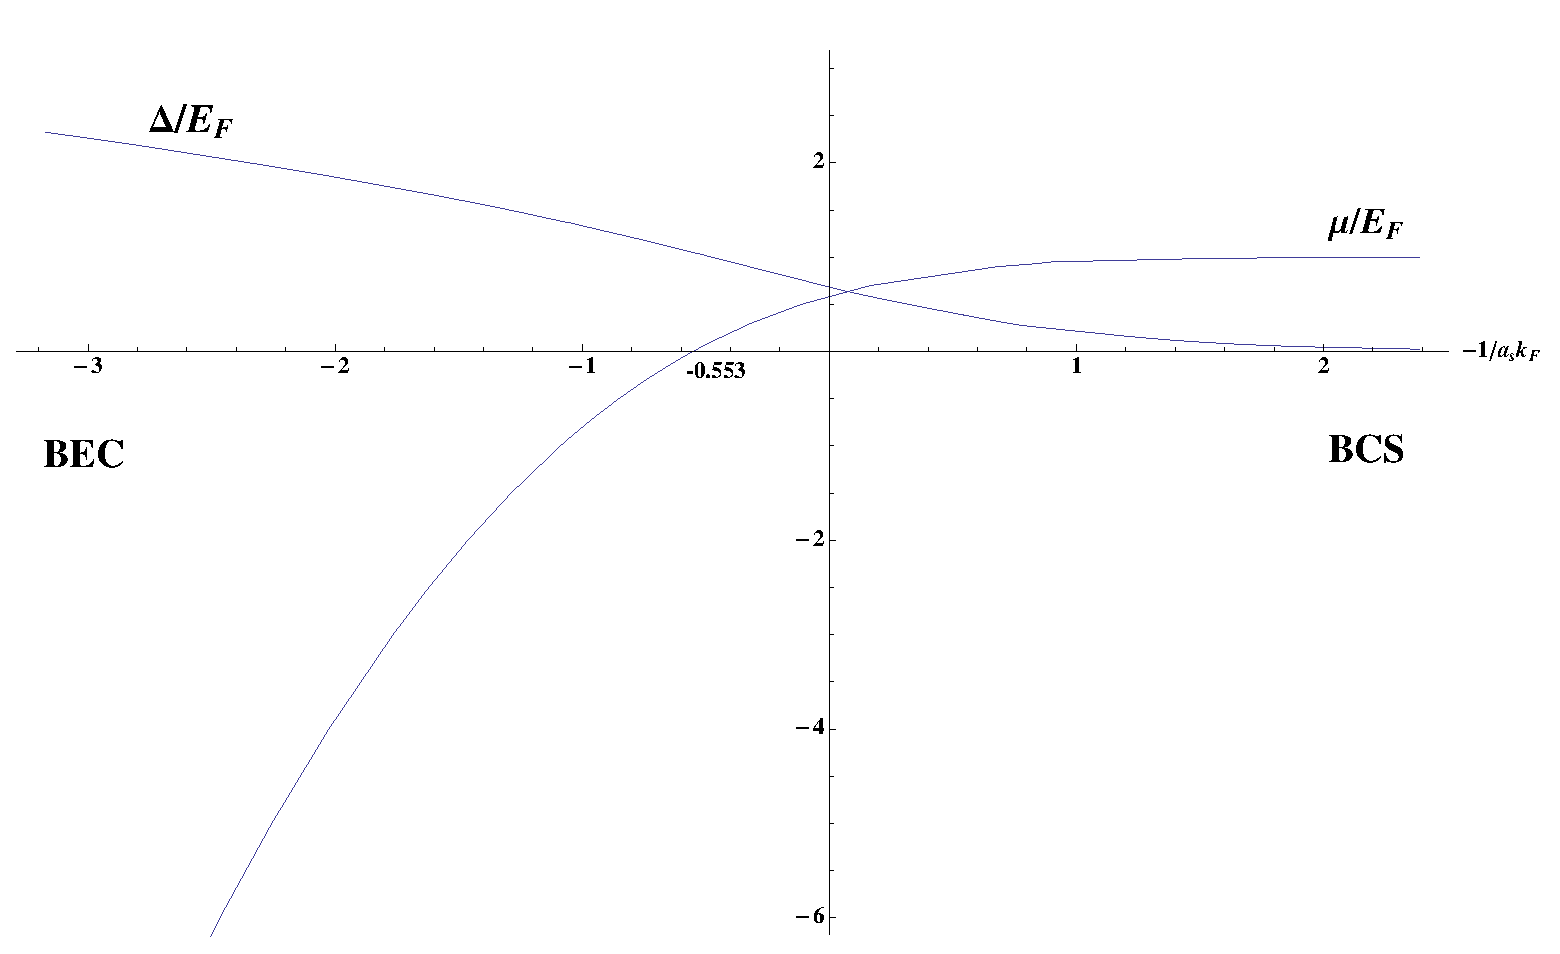
\includegraphics[width=0.8\textwidth]{SingleChannelCrossoverMuDelta}
\caption{The chemical potential $\mu$ and gap $\Delta$ in the mean field level over crossover} 
\label{fig:pathInt:meanField}
{\small All quantities in the unit of energy ($\mu$, $\Delta$) are rescaled with the Fermi energy $E_{F}$ and the s-wave scattering length $a_{s}$ is rescaled with $1/k_{F}$.  }
\end{center}
\end{figure}



\section{Gaussian fluctuation and collective modes}\label{sec:collective1}
We can expand the partition function Eq. (\ref{eq:pathInt:DeltaPF}) around the mean-field value, $\Delta(\vr,\tau)=\Delta_{0}+\theta(\vr,\tau)$. The linear order of the  expansion is zero because $\Delta_{0}$ is the saddle point.  The next order gives us the bilinear terms on $\theta$, i.e., correlation of bosonic fields $\Delta$ (four-fermion correlation).  Note that here the Hamiltonian only has a contact-type potential, therefore it cannot cover the situation of a charged system where long-range Columnb interaction cannot be neglected.  We limit ourselves to the neutual case.  Nevertheless, it is conceivable that a more realistic short-range potential only renormalizes some parameters in the following calculation while leaves the qualitative result unmodified.  

Notice that we can expand the second term in Eq. (\ref{eq:pathInt:DeltaPF}) for $\hat{G}{}^{-1}=\hat{G}_{0}^{-1}+\hat{K}$
\begin{equation}\label{eq:pathInt:expand}
\tr\ln \hat{G}^{-1}=\tr\ln\hat{G_{0}}^{-1}+\tr(\hat{G_{0}}\hat{K})-\nth{2}\tr(\hat{G_{0}}\hat{K}\hat{G_{0}}\hat{K})+\cdots
\end{equation}
In our case,
\begin{equation}
\hat{K}=\begin{pmatrix}
0&\theta\\
\theta^{*}&0
\end{pmatrix}
\end{equation}
Here the linear terms of $\hat{K}$ or $\theta$ ($\theta^{*}$) are zero as the saddle point condition.  To the second order, the action is 
\begin{equation}\label{eq:pathInt:DeltaActionGaussian}
S[\Delta_{0},\theta,\theta^{*}]=S[\Delta_{0}]+
	\nth{2g}\tr(\hat{K}\hat{K})+\nth{2}\tr(\hat{G_{0}}\hat{K}\hat{G_{0}}\hat{K})
\end{equation}
Write the last term into the momentum representation
\begin{equation}
\tr(\hat{G_{0}}\hat{K}\hat{G_{0}}\hat{K})=\sum_{q,p}\Tr\br{G_{0}({p})K_{q}G_{0}{}({p-q})K_{-q}}
\end{equation}
Notice that the second ``$\Tr$'' and following ``$\Tr$'' in this section only runs in Nambu spinor space and $q={(\vq,q_{l})}$, $p=(\vp,p_{n})$ are all four momentum, where $q_{l}$ is the bosonic Matsubara frequency while $p_{n}$ is the fermionic Matsubara frequency.
\begin{equation}
K_{p_{0},p_{0}+q}=K_{q}=\begin{pmatrix}
0&\theta_{q}\\
\theta^{*}_{-q}&0
\end{pmatrix}
\end{equation}
And we remember that $G_{0}(p)=G_{0}{}_{p,p}$
If we introduce  a new vector 
\begin{equation}
\theta{(q)}=\begin{pmatrix}\theta_{q}\\\theta^{*}_{-q}\end{pmatrix}\qquad
\theta^{\dg}{(q)}=\begin{pmatrix}\theta^{*}_{q}&\theta_{-q}\end{pmatrix}
\end{equation}
the action can be rewritten into a more compact form
\begin{equation}
S[\Delta_{0},\theta,\theta^{*}]=S[\Delta_{0}]+\nth{2}\sum_{q}\mbr{\theta^{\dg}(q)\mathbf{M}(q)\theta(q)}
\end{equation}
Notice that we can always choose a real $\Delta_{0}$ and therefore $G_{0}{\ _{12}}(p)=G_{0}{\ _{21}}(p)$, we have 
\begin{equation}
\mathbf{M}_{q,q}=\mathbf{M}(q)=
\begin{pmatrix}
\nth{g}+\sum_{p}G_{0}{\ }_{11}(p)G_{0}{\ }_{22}(p-q)&\sum_{p}G_{0}{\ }_{12}(p)G_{0}{\ }_{12}(p-q)\\
\sum_{p}G_{0}{\ }_{12}(p)G_{0}{\ }_{12}(p-q)&\nth{g}+\sum_{p}G_{0}{\ }_{11}(p-q)G_{0}{\ }_{22}(p)
\end{pmatrix}
\end{equation}
The summation over  the (fermionic) Matsubara frequency of $p_{n}$ can be carried out at zero temperature

\begin{equation}
\begin{split}
M_{11}(q)&=M_{22}(-q)\\
	&=\nth{g}+\sum_{\vp{,}p_{n}}G_{0}{\ }_{11}(p)G_{0}{\ }_{22}(p-q)\\
	&=\nth{g}+\sum_{\vp}\br{\frac{u^{2}u'^{2}}{iq_{l}-E-E'}-\frac{v^{2}v'^{2}}{iq_{l}+E+E'}}
\end{split}
\end{equation}
\begin{equation}
\begin{split}
M_{12}(q)&=M_{21}(q)\\
	&=\sum_{\vp{,}p_{n}}G_{0}{\ }_{12}(p)G_{0}{\ }_{12}(p-q)\\
	&=\sum_{\vp}uvu'v'\br{\nth{iq_{l}+E+E'}-\nth{iq_{l}-E-E'}}
\end{split}
\end{equation}
where $u=u_{\vp}$, $v=v_{\vp}$, $E=E_{\vp}$ and $u'=u_{\vp-\vq}$, $v'=v_{\vk-\vq}$, $E'=E_{\vk-\vq}$.  $u_{\vk}$, $v_{\vk}$, $E_{\vk}$ are as defined usually in BCS literature. 
\begin{equation}
v_{\vk}^{2}=1-u_{\vk}^{2}=\nth{2}\br{1-\frac{\xi_{\vk}}{E_{\vk}}}
\end{equation}
 The $G^{(M)}=\mathbf{M}^{-1}$ is the correlation function of $\theta$ (or $\Delta$) and its poles give the spectrum of collective modes as every  $\theta_{q}$ (or $\Delta_{q}$) involves many fermions moving in a coherent manner.  So the spectrum of collective modes can be determined by finding poles of $G^{(M)}$, $\det{M(\omega,\vq)}=0$ after we analytically continue for the frequency $iq_{l}\rightarrow\omega+i0^{+}$.  
 
For low energy modes, where $\omega,\,\abs{\vq}^{2}$ both are much smaller than $\min\bbr{E_{\vk}}=\Delta_{0}$ (or $\sqrt{\mu^{2}+\Delta^{2}}$ for $\mu<0$), we can expand $M$ with $\omega$ and $\vq$.  The lowest order has the form $\omega\approx{}c\,q$, which suggests a sound wave as expected for any Goldstone mode.  At BCS side, $c=v_{F}/\sqrt{3}$, where $v_{F}$ is Fermi velocity.  This coincides with the famous Anderson-Bogoliubov mode.  At the BEC side, we get $c^{2}=\Delta^{2}/8m\abs{\mu}=v_{F}^{2}(k_{F}a_{s})/3\pi=4\pi{}n_{B}a_{B}/m_{B}$, which fits the low momentum part of Bogoliubov spectrum of bosons gas.  Here $m_{B}=2m$ is the molecule mass, $n_{B}=n/2$ is the molecule density and $a_{B}=2a_{s}$ is the inferred  interaction between molecules.  This value differs from the result of more accurate calculation from the few-body theory, $a_{B}=0.6a_{s}$ \cite{Petrov}, which indicates the possible deficiency of the current theory. 


\section{An alternative method to invert the Green's function\label{sec:diagonalizeGreen1}}
In the above section, we inverted the  Gor'kov green function matrix Eqs. (\ref{eq:pathInt:nG}, \ref{eq:pathInt:G0}) directly and it is not hard to do as a $2\times2$ matrix in the  momentum space.   Alternatively, we can use a different approach which proves to be more convenient in the two-channel problem.  First, we diagonalize $\nG$ with a unitary transformation $T$, in the momentum space
\begin{equation}
\nG=\mtrx{i\omega_{n}-\xi_{k}&\Delta\\\bar\Delta&i\omega_{n}+\xi_{k}}=T^{\dg}BT
\end{equation}
It is easy to show that such $T$ and $B$ satisfying above equation are
\begin{equation}
T=\mtrx{u_{k}&v_{k}\\-v_{k}^{*}&u_{k}}\qquad{}B=\mtrx{i\omega_{n}+E_{k}&0\\0&i\omega_{n}-E_{k}}
\end{equation}
where $u_{k}^{2}(v_{k}^{2})=\nth{2}(1\pm\xi_{k}/E_{k})$ and $E_{k}=\sqrt{\xi^{2}_{\vk}+\Delta^{2}}$ are conventionally defined quantities in the BCS theory.   Actually, this transformation is nothing but the Bogoliubov canonical transformation, and the $B$ matrix simply describes the spectrum of the fermionic quasi-particles.  Now it is easy to invert $\nG$
\begin{equation}
\mathcal{G}=T^{\dg}B^{-1}T
\end{equation}
Green's function $\mathcal{G}$ takes a more conventional form $A/(i\omega_{n}\pm{}E_{k})$ without any dependency on frequency in nominator as Eq. (\ref{eq:pathInt:G0}). Matsubara frequency summation over $G_{0}(k)$ in the mean-field and $G_{0}(k)G_{0}(k+q)$ in the Gaussian order are then easier to perform  as in text-book.  


% !TeX root = subNote.tex

\subsection{Path integral approach for two-channel}
For two-channel problem, we write down the Hamiltonian as
\begin{equation}
\begin{split}
H&=\int{d^{d}r}\bigg\{\sum_{j}\bar\psi_{j}\mbr{\nth{2m}(-i\nabla)^{2}-\mu+\eta_{j}}\psi_{j}\\
	&\qquad-U\bar\psi_{a}(r)\bar\psi_{b}(r)\psi_{b}(r)\psi_{a}(r)-V\bar\psi_{a}(r)\bar\psi_{c}(r)\psi_{c}(r)\psi_{a}(r)\\
	&\qquad-\mbr{Y\bar\psi_{a}(r)\bar\psi_{b}(r)\psi_{b}(r)\psi_{a}(r)+h.c.}
	\bigg\}\\
 &=\int{d^{d}r}\bigg\{\sum_{j}\bar\psi_{j}\mbr{\nth{2m}(-i\nabla)^{2}-\mu+\eta_{j}}\psi_{j}
 	-(\bar\psi\bar\psi)\mtrx{U&Y\\Y^{*}&V}(\psi\psi)
\end{split}
\end{equation}
Here $\eta_{j}$ is the Zeeman energy of the specific hyperfine species.  a is the common species of two channels, (a,b) is the open channel and (a,c) is the close channel.  We can introduce a unitary transformation $Q$ (mixing two channels) to diagonalize the interaction matrix into diagonal matrix $A$.
\begin{equation}
Q^{\dg}AQ=\mtrx{U&Y\\Y^{*}&V}\equiv{}\tilde{U}
\end{equation}
The finite temperature action is 
\begin{equation}\label{eq:pathInt2:actionFermi}
S(\bar\psi,\psi)=\int^{\beta}_{0}d\tau\int{d^{d}r}\mbr{\sum_{j}\bar\psi_{j}(\partial_\tau-\nth{2m}\nabla^{2}-\mu+\eta_{j})\psi_{j}
-(\bar\psi\bar\psi)Q^{\dg}AQ(\psi\psi)}
\end{equation}

Now $(\psi\psi)$ is column vector and $(\bar\psi\bar\psi)$ is row vector
\begin{equation*}
(\bar\psi\bar\psi)=\mtrx{\bar\psi_{a}\bar\psi_{b}&\bar\psi_{a}\bar\psi_{c}}
\qquad(\psi\psi)=\mtrx{\psi_{b}\psi_{a}\\\psi_{c}\psi_{a}}
\end{equation*}

Similar as in Sec. \ref{sec:pathInt}, we can try to work on the two-channel problem.  Here, the bosonic field is a 2-component vector   and start from a fat identity
\begin{equation}\label{eq:pathInt2:indetity}
1=\int{D(\Delta,\bar\Delta)}\exp(-\int{dx}\Delta^{\dg}A^{-1}\Delta)
\end{equation}
here $x$ is four-coordinator,  $\int{dx}=\int^{\beta}_{0}d\tau\int{d^{d}r}$.  All the constant is absorbed into measure of functional integral of $D(\Delta,\bar\Delta)$.

\[
\Delta^{\dg}=(\bar\Delta_{1},\bar\Delta_{2})\qquad\Delta=\begin{pmatrix}\Delta_{1}\\\Delta_{2}\end{pmatrix}
\]
We can make a shift in $\Delta$
\begin{equation}
\Delta\longrightarrow\Delta-A\,Q(\psi\psi)
\end{equation}
Write it into the matrix form
\begin{equation*}
\mtrx{\Delta_{1}\\\Delta_{2}}\longrightarrow
	\mtrx{\Delta_{1}\\\Delta_{2}}-\mtrx{A_{11}&0\\0&A_{22}}\mtrx{Q_{11}&Q_{12}\\Q_{21}&Q_{22}}
	\mtrx{\psi_{b}\psi_{a}\\\psi_{c}\psi_{a}}
\end{equation*}
\begin{equation*}
\mtrx{\bar\Delta_{1},\bar\Delta_{2}}\longrightarrow
	\mtrx{\bar\Delta_{1},\bar\Delta_{2}}-
	\mtrx{\bar\psi_{a}\bar\psi_{b}&\bar\psi_{a}\bar\psi_{c}}
	\mtrx{Q_{11}^{*}&Q_{21}^{*}\\Q_{12}^{*}&Q_{22}^{*}}\mtrx{A_{11}&0\\0&A_{22}}
\end{equation*}

Note that in principle, $\bar{\Delta}_{i}$ is not simple complex conjugate of $\Delta_{i}$ as they are related to fermion field $\psi$ and $\bar\psi$, which are both Grassman numbers and is not relevant to each other.  But in our solution, we actually take them as complex conjugate.  Now the fat identity Eq. \ref{eq:pathInt2:indetity} becomes 
\begin{equation}
1=\int{D(\Delta,\bar\Delta)}\exp\big\{-\int{dx}
	[\Delta^{\dg}A^{-1}\Delta-(\bar\psi\bar\psi)Q^{\dg}\Delta-\bar\Delta{Q}(\psi\psi)+(\bar\psi\bar\psi)Q^{\dg}AQ(\psi\psi)]\big\}
\end{equation}
And we have 
\begin{equation}
\exp[\int{dx}(\bar\psi\bar\psi)Q^{\dg}AQ(\psi\psi)]
=\int{D(\Delta,\bar\Delta)}\exp\big\{-\int{dx}
	[\Delta^{\dg}A^{-1}\Delta-(\bar\psi\bar\psi)Q^{\dg}\Delta-\bar\Delta{Q}(\psi\psi)]\big\}
\end{equation}
This is ready to be apply to the original action in Eq. \ref{eq:pathInt2:actionFermi}, 
\begin{equation}\label{eq:pathInt2:actionMix}
S_{\tau}(\bar\Delta,\Delta,\bar\psi_{i},\psi_{i})=\int^{\beta}_{0}d\tau\int{d^{d}r}\bbr{\sum_{j}\bar\psi_{j}(\partial_\tau-\nth{2m}\nabla^{2}-\mu+\eta_{j})\psi_{j}
+[\Delta^{\dg}A^{-1}\Delta-(\bar\psi\bar\psi)Q^{\dg}\Delta-\bar\Delta{Q}(\psi\psi)}
\end{equation}
We can introduce a spinor space similar to Nambu spinor representation in single-channel superconductivity.  
\begin{equation}
\bar\Psi=\mtrx{\bar\psi_{a}&\psi_{b}&\psi_{c}}\qquad\Psi=\mtrx{\psi_{a}\\\bar\psi_{b}\\\bar\psi_{c}}
\end{equation}
the action can be rewritten in a more compact form
\begin{equation}\label{eq:pathInt2:actionMix}
S(\bar\Delta,\Delta,\bar\psi_{i},\psi_{i})=\int^{\beta}_{0}d\tau\int{d^{d}r}
	\mbr{\bar\Delta{}A^{-1}\Delta-\bar\Psi\mathcal{G}^{-1}\Psi}
\end{equation}
where 
\begin{equation}
\mathcal{G}^{-1}=
\begin{pmatrix}
-\partial_{\tau}+\nth{2m}\nabla^{2}+\mu-\eta_{a}&Q^{*}_{11}\Delta_{1}+Q^{*}_{21}\Delta_{2}&Q^{*}_{12}\Delta_{1}+Q^{*}_{22}\Delta_{2}\\
Q^{}_{11}\bar\Delta_{1}+Q^{}_{21}\bar\Delta_{2}&-\partial_{\tau}-\nth{2m}\nabla^{2}-\mu+\eta_{b}&0\\
Q^{}_{12}\bar\Delta_{1}+Q^{}_{22}\bar\Delta_{2}&0&-\partial_{\tau}-\nth{2m}\nabla^{2}-\mu+\eta_{c}
\end{pmatrix}
\end{equation}
The action is now bilinear to $\Psi$ and we can integrate it out formally
\begin{equation}
S(\bar\Delta,\Delta)=\int{dx}
	\br{\bar\Delta{}A^{-1}\Delta-\tr\ln{G}^{-1}}
\end{equation}
This form can be simplified by introducing mixture within two channels.
\begin{equation}
D\equiv\mtrx{D_{1}\\D_{2}}=Q^{\dg}\Delta
\end{equation}

We furthermore assume $\eta_{a}=\eta_{b}=0$, $\eta_{c}=\eta$. In frequency-momentum space, 
\begin{equation}\label{eq:pathInt2:nG}
\mathcal{G}^{-1}=i\omega_{n}I+
\begin{pmatrix}
-\xi_{k}&D_{1}&D_{2}\\
\bar{D}_{1}&+\xi_{k}&0\\
\bar{D}_{2}&0&+\xi_{k}+\eta
\end{pmatrix}
\end{equation}
here $\xi_{k}=\nth{2m}k^{2}-\mu$; and 
\begin{equation*}
\bar\Delta=\bar{D}\,Q^{\dg}\qquad\Delta=Q\,D
\end{equation*}
\[
\bar\Delta{}A^{-1}\Delta=\bar{D}Q^{\dg}A^{-1}QD=\bar{D}\tilde{U}^{-1}D
\]
Now we can change the functional variable into $D(\bar{D})$ 
\begin{equation}\label{eq:pathInt2:actionD}
S(\bar{D},D)=\int{dx}\br{\bar{D}\tilde{U}^{-1}D-\tr\ln{G}^{-1}}
\end{equation}
Comparing Eq. \ref{eq:pathInt2:nG} with Eq. \ref{eq:canonical:M} in Bogoliubov transformation treatment, we  see that $D_{1,2}$ have simple physical meaning in the mean-field expression of $\nG_{0}$ and therefore are more  direct counterpart of order parameter $\Delta$ in single-channel problem. 



\subsubsection{Diagonalize Green's function, Fermionic mode and Bogoliubov transform\label{sec:diagonalGreen}}
Here we will use the approach in Sec. \ref{sec:diagonalizeGreen1} for our problem.  In current problem, we need to diagonalize a $3\times3$ matrix Eq. \ref{eq:pathInt2:nG}, in another word, we need to figure out the Bogoliubov canonical transformation and the quasiparticle spectrum for this problem.   This involves solving a cubic equation, and an exact solution exists in principle.  However,  it offers little intuition in write the exact result, instead we content to find the approximated result when spectrum does not change too much from the broad-resonance, where the only effect of close-channel is modifying the effective interaction of open-channel. 


Within the assumption that spectrum  deviates not too much from na\"{i}ve broad-resonance solution, we  break down the unitary transformation into two 
pieces. 
\begin{equation}
B_k=L_k^{\dg}T_k^{\dg}G_k^{-1}T_kL_k
\end{equation} 
Here $T$ and $L$ are both unitary transformation.  We take $T$ as the transformation at lowest order, i.e., when we can ignore Pauli exclusion between channels. 
\begin{equation}
T_k=\mtrx{u_k&v_k&0\\-v_k&u_k&0\\0&0&1}
\end{equation}
Here we define 
\begin{gather}
E_{\vk}=(\xi_{\vk}^{2}+D_{1}^{2})^{1/2}\\
v_{\vk}^{2}=1-u_{\vk}^{2}=\nth{2}\br{1-\frac{\xi_{\vk}}{E_{\vk}}}
\end{gather}

In the broad-resonance, $L$ is simply identity matrix.  Here we will try to approximate it to the first order correction due to Pauli exclusion between two-channel.  
Apply $T_k$ onto $G^{-1}$, we have 
\begin{equation}\label{eq:pathInt2:G2}
T_k^{\dg}G_k^{-1}T_k=i\omega_nI+\mtrx{-E_k&0&u_kD_2\\0&+E_k&v_kD_2\\u_kD_2&v_kD_2&+\xi_k+\eta}
\end{equation}
We regard the off-diagonal elements as perturbation.  This matrix can then be diagonalized with another unitary transformation $L_{\vk}$ within the first order of $D_{i}^{2}/(E\eta)$
\begin{equation}
\begin{split}
B_{\omega_{n},\vk}&=i\omega_{n}I-
	\mtrx{\xi_{1}{}_{\vk}&0&0\\0&\xi_{2}{}_{\vk}&0\\0&0&\xi_{3}{}_{\vk}}\\
	&\approx{}i\omega_{n}I+
	\mtrx{-E_{\vk}-\frac{D_{1}^{2}}{\eta}&0&0\\
	0&E_{\vk}-\frac{D_{2}^{2}}{\eta}&0\\0&0&\xi_{\vk}+\eta+\frac{D_{1}^{2}+D_{2}^{2}}{2\eta}}
%	&=
%	\mtrx{i\omega_{n}-E_{\vk}&0&0\\0&i\omega_{n}+E_{\vk}&0\\0&0&i\omega_{n}+\eta}
%	+\mtrx{-\frac{D_{1}^{2}}{\eta}&0&0\\0&-\frac{D_{2}^{2}}{\eta}&0\\0&0&+\frac{D_{1}^{2}+D_{2}^{2}}{2\eta}}\\
%	&\equiv{}B^{(0)}_{\vk}+B^{(1)}_{\vk}
\end{split}	
\end{equation}
\begin{equation}\label{eq:pathInt2:L1}
L_{\vk}\approx{}I+
\mtrx{0&-\frac{D_{1}{}D_{2}{}}{4E^{2}_{\vk}}&u_{\vk}\\
\frac{D_{1}{}D_{2}{}}{4E^{2}_{\vk}}&0&v_{\vk}\\
-u_{\vk}&-v_{\vk}&0
}\frac{D_{2}{}}{\eta}
\equiv{}I+\delta_{k}\qquad
L^{\dg}_{\vk}=I-\delta_{\vk}
\end{equation}
Here we use $uv=D_{1}/2E$.  Please see Appendix \ref{sec:diagonalize} for details.  Note that $L$ and $L^{\dg}$ are unitary only to the first order of $D_{i}/\eta$
And now it is easy to express the Green's function
\begin{equation}
G_{\vk}=T_{\vk}L_{\vk}B_{\vk}^{-1}L_{\vk}^{\dg}T_{\vk}^{\dg}
\end{equation}
This is ready to be expanded over the perturbation in order of  $D_{i}^{2}/(E\eta)$ or $D_{i}/\eta$.  It is easy to see that all $\omega_{n}$ dependence concentrates on $B_{\vk}$, which simplifies the Matsubara frequency summation considerably.   
\begin{equation}\label{eq:pathInt2:Gexpand}
G_{k}=T_{\vk}B_{\omega_{n},\vk}^{-1}T_{\vk}^{\dg}+T_{\vk}\delta_{\vk}B_{\omega_{n},\vk}^{-1}T_{\vk}^{\dg}
	-T_{\vk}B_{\omega_{n},\vk}^{-1}\delta_{\vk}T_{\vk}^{\dg}=G_{\vk}^{(0)}+G_{\vk}^{(1)}
\end{equation}

From another point, we can interprate the above transform $T_\vk{}L_\vk$ as Bogoliubov canonical transformation and $B$ gives us spectrum of fermionic quasi-particle excitation.  
%We only need to keep the zeroth order term for $B_{\vk}^{-1}$ for first order expansion.  

\subsubsection{Mean field result}
 Use the same techniques as Eq. (\ref{eq:pathInt:diffTr}), we have two equations for $D_{1}$ and $D_{2}$,
 \begin{align}
\frac{\delta}{\delta{}D_{1}}:&\qquad&
(\tilde{U}^{-1})_{11}\bar{D}_{1}+(\tilde{U}^{-1})_{21}\bar{D}_{2}-\tr\mbr{{G_{0}}\cdot\cmtrx{0&1&0\\0&0&0\\0&0&0}}=0\\
\frac{\delta}{\delta{}D_{2}}:&\qquad&
(\tilde{U}^{-1})_{12}\bar{D}_{1}+(\tilde{U}^{-1})_{22}\bar{D}_{2}-\tr\mbr{{G_{0}}\cdot\cmtrx{0&0&1\\0&0&0\\0&0&0}}=0
 \end{align}


 If we take $D$ as real constant\footnote{Actually $D_{2}{_{\vk}}$ cannot be constant at high momentum.  However, for the momentum we are interested, i.e. the momentum lower or in the order of Fermi momentum, it slowly varies.  Therefore fairly it is reasonable to take it as constant.},     we can find the mean field result.  Usting Eq. (\ref{eq:pathInt2:Gexpand}),
 
 \begin{equation}\label{eq:pathInt2:G0}
 \begin{split}
 G_{0}=&
 \begin{pmatrix}
 {g_{1\,\vk}}&
-u_{k}v_{k}{g_{2\,\vk}}&0\\
-u_{k}v_{k}{g_{2\,\vk}}& {g_{3\,\vk}}&0\\
  0&0&\nth{i\omega_{n}-\xi_{3}{}_{\vk}}
 \end{pmatrix}\\
&+\frac{D_{2}}{\eta}
\begin{pmatrix}
\frac{D_{1}^{2}D_{2}}{4E_{\vk}^{3}}g_{2\,\vk}&\frac{D_{1}D_{2}\xi_{\vk}}{4E_{\vk}^{3}}g_{2\,\vk}&-g_{1\,\vk}+\nth{i\omega_{n}-\xi_{3}{}_{\vk}}\\
\frac{D_{1}D_{2}\xi_{\vk}}{4E_{\vk}^{3}}g_{2\,\vk}&-\frac{D_{1}^{2}D_{2}}{4E_{\vk}^{3}}g_{2\,\vk}&u_{k}v_{k}{g_{2\,\vk}}\\
-g_{1\,\vk}+\nth{i\omega_{n}-\xi_{3}{}_{\vk}}&u_{k}v_{k}{g_{2\,\vk}}&0
\end{pmatrix}
\end{split}
 \end{equation}
\begin{gather}
g_{1}{}_{\vk}=\frac{u_{\vk}^{2}}{i\omega_{n}-\xi_{1}{}_{\vk}}+\frac{v_{\vk}^{2}}{i\omega_{n}-\xi_{2}{}_{\vk}}\\
g_{2}{}_{\vk}=\nth{i\omega_{n}-\xi_{1}{}_{\vk}}-\nth{i\omega_{n}-\xi_{2}{}_{\vk}}\\
g_{3}{}_{\vk}=\frac{v_{\vk}^{2}}{i\omega_{n}-\xi_{1}{}_{\vk}}+\frac{u_{\vk}^{2}}{i\omega_{n}-\xi_{2}{}_{\vk}}
\end{gather}

 \begin{align*}
\tr\mbr{G_{0}\cdot\cmtrx{0&1&0\\0&0&0\\0&0&0}}&=
\sum_{\omega_{n}}\sum_{\vk}
	\mbr{(\nth{i\omega_{n}-\xi_{1}{}_{\vk}}-\nth{i\omega_{n}-\xi_{2}{_{\vk}}})
	(-\frac{D_{1}}{2E_{\vk}}+\frac{D_{1}D_{2}^{2}\xi_\vk}{4E_{\vk}^{3}\eta})}\\
	&=\sum_{\vk}(\frac{D_{1}}{2E_{\vk}}-\frac{D_{1}D_{2}^{2}\xi_\vk}{4E_{\vk}^{3}\eta})\\
\tr\mbr{G_{0}\cdot\cmtrx{0&0&1\\0&0&0\\0&0&0}}&=
\sum_{\omega_{n}}\sum_{\vk}
\mbr{\nth{i\omega_{n}-\xi_{3}{}_{\vk}}-
\frac{u_{\vk}^{2}}{i\omega_{n}-\xi_{1}{}_{\vk}}-\frac{v_{\vk}^{2}}{i\omega_{n}-\xi_{2}{}_{\vk}}}\frac{D_{2}}{\eta}\\
&=\sum_{\vk}\frac{D_{2}}{\eta}u_{\vk}^2
  \end{align*}
Here we take the interest only in $T=0$, so we only need to consider the negative frequencies ($\xi_{2\,\vk}$, $\xi_{3\,\vk}$) for summation of Matsubara frequency. Note that the second summation diverges badly in high-momentum. %this is because we take $D_2$ as constant.  It decreases at high-energy in the scale of $\eta$ and needs to be regularize carefully.  
We notice that this term is controlled by parameter $D_{2}/\eta$, this actually goes back to the fact that we only keep the first order in $L$ expansion (Eq. \eqref{eq:pathInt2:L1}), which is only valid for energy smaller or in order of Fermi energy.  In a more careful study, this term should be like $D_{2}/(\epsilon_{k}+\eta)$, is approximately $D_{2}/\eta$ when the interesting region  is lower or at the Fermi energy.   We can reestablish the $F_{k}\propto1/\epsilon_{k}$ if we retain all terms in the expansion of $L$, i.e. inverting Green's function $G$ exactly.       Indeed it should be just proportional to simple bounded two-body solution of isolated close-channel, $\phi_{0\,\vk}$ at high-momentum, which is not of interest for the many-body problem. 
 Another interesting thing about this term is the $u_\vk$ factor, which is small below chemical potential $\mu$ in BCS side.  This shows the fact that the low momentum is filled mostly by open-channel and close-channel is crowded out.  However, this does not affect close-channel too much as it is much more extended in momentum space and its occupation over each level is low due to the smaller size of close-channel bound state.  With above result, we can rewrite gap equations as 
\begin{equation*}
\tilde{U}^{-1}D-\mtrx{\sum_{\vk}(\frac{D_{1}}{2E_{\vk}}-\frac{D_{1}D_{2}^{2}\xi_\vk}{4E_{\vk}^{3}\eta})\\\sum_{\vk}\frac{D_{2}}{\eta}u_{\vk}^2}=0
\end{equation*}
 We can multiply it with $\tilde{U}$ and we have 
\begin{equation}\label{eq:pathInt2:meanfield}
\mtrx{D_1\\D_2}=\mtrx{U&Y\\Y^{*}&V}\sum_{\vk}\mtrx{\frac{D_{1}}{2E_{\vk}}-\frac{D_{1}D_{2}^{2}\xi_\vk}{4E_{\vk}^{3}\eta}\\
\frac{D_{2}}{\eta}u_{\vk}^2}
\end{equation}
 This equation can be renormalized in a very similar fashion as variation method. Notice that the second term in the first component describes the Pauli exclusion between two channels.  

\subsection{Renormalizing mean-field equation}
We define two quantities for the summand in the mean-field equation Eq. \ref{eq:pathInt2:meanfield}.
\begin{gather}
F_{1\,\vk}=\frac{D_{1}}{2E_{\vk}}-\frac{D_{1}D_{2}^{2}\xi_\vk}{4E_{\vk}^{3}\eta}\\
F_{2\,\vk}=\frac{D_{2}}{\eta}u_{\vk}^2\label{eq:pathInt2:F2k}
\end{gather}
Considering the argument from last section, we modify equation of $F_2$ to the following,
\begin{equation}
\tilde{F}_{2\,\vk}=\frac{D_{2}}{\eta+2\epsilon_{\vk}}u_{\vk}^2\label{eq:pathInt2:F2kMod}
\end{equation}
And now $F_2$ has the same behavior at high momentum as $F_1$, actually this is the behavior we expected for $\epsilon_k<\eta$, it falls off even faster beyond energy scale of $\eta$, which is determined by the specific shape of close-channel potential.

We can rewrite the mean-field equation as
\begin{gather}
D_{1}=\sum_{\vk}(U F_{1\,\vk}+Y \tilde{F}_{2\,\vk})\label{eq:pathInt2:D2}\\
D_{2}=\sum_{\vk}(Y^{*} F_{1\,\vk}+V \tilde{F}_{2\,\vk})\label{eq:pathInt2:D2}
\end{gather}
Here we see the $F_{1\,\vk}$ and $\tilde{F}_{2}$  both go as $1/\epsilon_{\vk}$  at high-momentum.  %To resolve divergence in the summation of $F_{2\,\vk}$ we restore the momentum dependence on $D_{2\,\vk}$ and therefore $F_{2\,\vk}$.  
  And we can see $\frac{D_{2}}{\eta}$ is actually a good approximation at low-momentum, where kinetic energy is much smaller than $\eta$.  We can rewrite $\tilde{F}_{2}=\alpha\phi_{0\,\vk}u_{\vk}^{2}$. Eq. (\ref{eq:pathInt2:D2}) can be rewritten as
\begin{equation*}
\eta{}F_{2\,\vp}=\sum_{\vk}(Y^{*} F_{1\,\vk}+V F_{2\,\vk})\label{eq:pathInt2:D2}
\end{equation*}
comparing this to a two-body \sch equation
\begin{equation*}
-E_{0}\phi_{0\,\vp}=\epsilon_{\vp}\phi_{0\,\vp}-\sum_{\vk}V \phi_{0\,\vk}\label{eq:pathInt2:D2}
\end{equation*}
where $E_{0}$ is the binding energy of two-body bound state of isolated close-channel.   


\subsection{Collective mode}
%\subsection{Simple approach for collective mode}
With the above arrangement, it is easy to study the collective mode of the system, which corresponding the second order expansion over $D$. We introduce the deviation over $\nG=G_{0}^{-1}+K_{q}$, where $G_{0}$ is described by real constant $D_{1,2}$
\begin{equation}
K_\vq=\mtrx{0&\theta_{1\,\vq}&\theta_{2\,\vq}\\\theta_{1\,-\vq}^*&0&0\\\theta_{2\,-\vq}^*&0&0}
\end{equation}
Follow the same approach in single-channel (Sec. \ref{sec:collective1}), we need to calculate $\tr(\hat{G_{0}}\hat{K}\hat{G_{0}}\hat{K})$, 
\begin{equation}
\tr({G_{0\,k}}{K_{q}}{G}_{0\,k+q}{K_{-q}})=\Theta_{q}^{\dg}M_{q}\Theta_{q}
\end{equation}
where 
\begin{equation}
\Theta_{q}=\mtrx{\theta^{*}_{1\,\vq}\\\theta^{}_{1\,-\vq}\\\theta^{*}_{2\,\vq}\\\theta^{}_{2\,-\vq}}
\qquad
\Theta_{q}^{\dg}=\mtrx{\theta^{}_{1\,\vq}&\theta^{*}_{1\,-\vq}&\theta^{}_{2\,\vq}&\theta^{*}_{2\,-\vq}}
\end{equation}
At the lowest order, if we take $L_{\vq}=I$,
\begin{equation}
M^{(0)}_{q}=\sum_{\vk}
\begin{pmatrix}
-u_{\vk}^{2}u_{\vk+\vq}^{2}f_{1\,q}+v_{\vk}^{2}v_{\vk+\vq}^{2}f_{2\,q}&u_{\vk}v_{\vk}u_{\vk+\vq}v_{\vk+\vq}(f_{2\,q}-f_{1\,q})&0&0\\
u_{\vk}v_{\vk}u_{\vk+\vq}v_{\vk+\vq}(f_{2\,q}-f_{1\,q})&u_{\vk}^{2}u_{\vk+\vq}^{2}f_{2\,q}-v_{\vk}^{2}v_{\vk+\vq}^{2}f_{1\,q}&0&0\\
0&0&-u_{\vk}^{2}f_{3\,q}&0\\
0&0&0&u_{\vk+\vq}^{2}f_{4\,q}
\end{pmatrix}
\end{equation}
where
\begin{gather}
f_{1\,q}=\nth{i q_{l}+\xi_{1\,\vk}-\xi_{2\,\vk+\vq}}\\
f_{2\,q}=\nth{i q_{l}-\xi_{1\,\vk+\vq}+\xi_{2\,\vk}}\\
f_{3\,q}=\nth{i q_{l}+\xi_{1\,\vk}-\xi_{3\,\vk+\vq}}\\
f_{4\,q}=\nth{i q_{l}-\xi_{1\,\vk+\vq}+\xi_{3\,\vk}}
\end{gather}
The two channels are completely decoupled at this level and the upper quarter is exactly same as single channel case if we ignore the correction over quasi-particle spectrum.   We can also expand each $f_{i\,q}$ to get the first order about $D_{2}/\eta$. (We take $q=0$ for it. See Appendix \ref{sec:expansionM})
\begin{equation}
M^{(1a)}=\sum_{\vk}
\begin{pmatrix}
(1-\frac{D_{1}^{2}}{2E_{\vk}^{2}})\frac{D_{1}^{2}-D_{2}^{2}}{4E_{\vk}^{2}\eta}
&-\frac{D_{1}^{2}}{4E_{\vk}^{2}}\frac{D_{1}^{2}-D_{2}^{2}}{4E_{\vk}^{2}\eta}&0&0\\
-\frac{D_{1}^{2}}{4E_{\vk}^{2}}\frac{D_{1}^{2}-D_{2}^{2}}{4E_{\vk}^{2}\eta}
&(1-\frac{D_{1}^{2}}{2E_{\vk}^{2}})\frac{D_{1}^{2}-D_{2}^{2}}{4E_{\vk}^{2}\eta}&0&0\\
0&0&\nth{2}(1+\frac{\xi_{\vk}}{E_{\vk}})\frac{3D_{1}^{2}+D_{2}^{2}}{2\eta(E_{\vk}+\xi_{\vk}+\eta)}&0\\
0&0&0&\nth{2}(1+\frac{\xi_{\vk}}{E_{\vk}})\frac{3D_{1}^{2}+D_{2}^{2}}{2\eta(E_{\vk}+\xi_{\vk}+\eta)}
\end{pmatrix}
\end{equation}

To be consistent, we also need to expand $L_{q}$ to the first order of  $D_{2}/\eta$ as well.  
\begin{equation}
\begin{split}
M^{(1b)}=&\qquad\frac{D_{2}}{\eta}\sum_{\vk}\\
&\begin{pmatrix}
-\frac{D_{1}^{2}D_{2}\xi_{\vk}}{4E^{5}_{\vk}}&-\frac{D_{1}^{2}D_{2}\xi_{\vk}}{2E^{5}_{\vk}}
&\frac{D_{1}\xi_{\vk}}{4E_{\vk}^{3}}&\frac{D_{1}}{2E_{\vk}}(\nth{E_{\vk}+\xi_{\vk}+\eta}+\nth{2E_{\vk}})\\
-\frac{D_{1}^{2}D_{2}\xi_{\vk}}{4E^{5}_{\vk}}&-\frac{D_{1}^{2}D_{2}\xi_{\vk}}{2E^{5}_{\vk}}
&\frac{D_{1}}{2E_{\vk}}(\nth{E_{\vk}+\xi_{\vk}+\eta}+\nth{2E_{\vk}})&\frac{D_{1}\xi_{\vk}}{4E_{\vk}^{3}}\\
\frac{D_{1}\xi_{\vk}}{4E_{\vk}^{3}}&\frac{D_{1}}{2E_{\vk}}(\nth{E_{\vk}+\xi_{\vk}+\eta}+\nth{2E_{\vk}})
&-\frac{D_{1}^{2}D_{2}}{4E_{\vk}^{3}(E_{\vk}+\xi_{\vk}+\eta)}&0\\
\frac{D_{1}}{2E_{\vk}}(\nth{E_{\vk}+\xi_{\vk}+\eta}+\nth{2E_{\vk}})&\frac{D_{1}\xi_{\vk}}{4E_{\vk}^{3}}
&0&-\frac{D_{1}^{2}D_{2}}{4E_{\vk}^{3}(E_{\vk}+\xi_{\vk}+\eta)}\\
\end{pmatrix}
\end{split}
\end{equation}
The interesting thing here is that if we only takes the first order of $D_{2}/\eta$, the two-channel is still decoupled when we write down the secular equation.  And the correction of the elements at the upper-left corner ($\theta_{1\,\pm{q}}$) is the same and that will gives an small finite value for $\omega_{q}$ at $q=0$. \emph{This conclusion is however problemetic as it violates the f sum rule.  Phase flucturation should be a Goldstone mode without mass.(see Sec. \ref{sec:phaseFluctuation}) }

\subsubsection{Alternative Approach: Phase fluctuation mode \label{sec:phaseFluctuation}}
 Action of $D$, $S(\bar{D_i},D_i)$ Eq. \eqref{eq:pathInt2:nG} and Eq. \eqref{eq:pathInt2:actionD}, is invariant over the phase change of $D_{1\,\vk}$ and $D_{2\,\vk}$ simultaneously. We therefore conclude that we should have a massless (Goldstone) mode.  And particularly, this mode is related to the local phase invariance. 
\begin{equation*}
D_{i}(x)\rightarrow{}D_{i}(x)e^{i2\theta(x)}\qquad{}
\bar{D}_{i}(x)\rightarrow{}\bar{D}_{i}(x)e^{-i2\theta(x)}
\end{equation*}
This corresponding to the translation of fermionic operator $\psi$
\begin{equation*}
\psi_{i}(x)\rightarrow{}\psi_{i}(x)e^{i\theta(x)}\qquad{}
\bar{\psi}_{i}(x)\rightarrow{}\bar{\psi}_{i}(x)e^{-i2\theta(x)}
\end{equation*}
Note that the phase $\theta(x)$ is common for the different components. The rest three degree of freedom of $D_i$, magnitude variation of two $D_i$ and internal phase between two $D_i$, change the action accordingly, while the overall phase $\theta(x)$ leaves action invariant.  We here isolate this special degree of freedom while leave others at their mean-field values. With a phase shift, we can rewrite the action (taken mean-field value $D^{(0)}$) (here we closely follow Nagaosa\cite{Nagaosa})
\begin{subequations}
\begin{align}\label{eq:pathInt2:actionPhase}
S[\theta,\bar\psi_{i},\psi_{i}]=&S_0[\bar\psi_{i},\psi_{i}]+S_1[\theta,\bar\psi_{i},\psi_{i}]+S_2[\theta,\bar\psi_{i},\psi_{i}]\\
S_0[\bar\psi_{i},\psi_{i}]=&\int{dx}
\Big\{\sum_{j}\bar\psi_{j}(\partial_\tau-\nth{2m}\nabla^{2}-\mu+\eta_{j})\psi_{j}\nonumber\\
&\quad+[D^{(0)}{}^{\dg}\tilde{U}^{-1}D^{(0)}-(\bar\psi\bar\psi)D^{(0)}-{D^{(0)}}{}^{\dg}(\psi\psi)\Big\}\\
S_1[\theta,\bar\psi_{i},\psi_{i}]=&\int{dx}\sum_{j}\Big\{
   i\,\bar\psi_{j}(\partial_{\tau}\theta)\psi_{j}+\nabla\theta\cdot\nth{2mi}[\bar\psi_{j}\nabla\psi_{j}-(\nabla\bar{\psi}_{j}\psi_{j})]\Big\}\\
S_2[\theta,\bar\psi_{i},\psi_{i}]=&\int{dx}\sum_{j}\nth{2m}(\nabla\theta)^{2}\bar\psi_{j}\psi_{j}
\end{align}
\end{subequations}
Note that here $D^{(0)}$ is a constant 2-component vector, no longer functional variables.  Here we see that $S_{0}$ has the same form as before except it only takes the mean field value of $D$ and it is described by the same correlation $G_{0}$ (Eq. \eqref{eq:pathInt2:G0}, \eqref{eq:pathInt2:nG}).  We can regard $S_{1}$ and $S_{2}$ as perturbation for the so-called gradient expansion on $\nabla\theta$.  It is then obvious that $S_{1}$ is in the first order while $S_{2}$ is in the second order.  Use the same spinor representation as before, $S$ is bilinear of $\psi$ and therefore we can formally integrate out $\psi$. 
\begin{equation}
S[\theta]=const.+\ln\det\nG(\theta)
\end{equation}
 We write out the formal Green function according to above action (with respect to Nambu-like spinor)
\begin{subequations}
\begin{align}
\nG=&G_{0}^{-1}+K_{1}+K_{2},\\
K_{1\, k,k'}=
	&\nth{({\beta{}V)}^{1/2}}(\omega_n-\omega_{n'})\theta(k-k')\sigma_3+
		\nth{{(\beta{}V)}^{1/2}}i\frac{(\vk-\vk')\cdot(\vk+\vk')}{2m}\theta(k-k')\hat{1}\\
K_{2\, k,k'}=
	&\nth{2m}\sum_{q,q'}\nth{{\beta{}V}}(\vq\cdot\vq')\theta(q)\theta(q')\delta(q+q'+k-k')\sigma_3
\end{align}
\end{subequations}
where $G_{0}$ is the same as (Eq. \eqref{eq:pathInt2:G0}, \eqref{eq:pathInt2:nG}).  And like in the single channel, 
\begin{equation}
\sigma_3=\mtrx{1&0&0\\0&-1&0\\0&0&-1}
\end{equation}
and $\hat{1}$ is $3\times3$ identity matrix.  As the expansion in Eq. \ref{eq:pathInt:expand}, we can look for the expansion of $\nG$ over $K_{1,2}$.  
\begin{equation}\tag{\ref{eq:pathInt:expand}}
\tr\ln \hat{G}^{-1}=\tr\ln\hat{G_{0}}^{-1}+\tr(\hat{G_{0}}\hat{K})-\nth{2}\tr(\hat{G_{0}}\hat{K}\hat{G_{0}}\hat{K})+\cdots
\end{equation}
For the first order, $\tr(\hat{G_{0}}\hat{K})$, 
\begin{align}
\tr(\hat{G_{0}}\hat{K_1})=&\sum_{k}{G_{0\,k}K_{1\,k,k}}=0\\
\tr(\hat{G_{0}}\hat{K_2})=&\sum_{k}{G_{0\,k}K_{2\,k,k}}\nonumber\\
	=&-\nth{2m}\nth{{\beta{}V}}\sum_{k}\tr(\hat{G}_{0\,k}\sigma_3)\sum_{q}q^2\theta{q}\theta{-q}\nonumber\\
	=&-\frac{n}{2m}\sum_{q}q^2\theta{(q)}\;\theta{(-q)}
\end{align}
Here we use the fact $\nth{{\beta{}V}}\sum_{k}\tr(\hat{G}_{0\,k}\sigma_3)=n$. $\tr(\hat{G_{0}}\hat{K_2})$ is already in the second order of $\theta$, and we only need to keep the expansion of $K_2$ to this order. On the other hand, we have to go to the second order of $K_1$ for the second order of $\theta$. 
\begin{align}		
\tr(\hat{G_{0}}{K_1}\hat{G_{0}}{K_1})=&\sum_{k,q}\tr(\hat{G}_{0,k+q}K_{1\,k+q,k}\hat{G}_{0\,k}K_{1\,k,k+q})\\
=&\nth{{\beta{}V}}\sum_{k,q}\theta(q)\theta(-q)\Big[(-\omega_m^2)\tr(\hat{G}_{0,k+q}\sigma_3\hat{G}_{0\,k}\sigma_3)\nonumber\\
&\quad+\nth{m^2}\sum_{i,j}q_iq_j(k_i+\frac{q_i}{2})(k_j+\frac{q_j}{2})\tr(\hat{G}_{0,k+q}\hat{G}_{0\,k})\Big]\nonumber\\
\equiv&\sum_{q}\theta(q)\theta(-q)\big[-\pi^{(0)}(q)\omega_m^2+\sum_{ij}\pi^{(\perp)}_{ij}(q)q_iq_j\big]
\end{align}
\emph{Here we only interested in the low-energy behavior of the mode and therefore we only use $\pi(0)$.} Use the previous result of Sec. \ref{sec:diagonalGreen}, we can calculate the Green's function in the lowest and first order of $D_i/\eta$ in $\pi$.  After some long but straigh-forward algebra (see Sec. \ref{sec:calculatePi}), we find
\begin{gather}
\pi^{(0)}(0)\approx\sum_{\vk}\frac{D_{1}^{2}}{E_{\vk}^{3}}-(\frac{D_{1}^{2}+D_{2}^{2}}{2\eta})\sum_{\vk}\frac{D_{1}^{2}}{E_{\vk}^{4}}\\
\pi^{(\perp)}(0)=0
\end{gather}
Combine all these together
\begin{equation}
S[\theta]=\int{dx}\sum_{q}\theta(q)\theta(-q)\big[\nth{2}\pi^{(0)}(q)\omega_m^2-\frac{n}{2m}q^2\big]
\end{equation}
And this determines the velocity of the Anderson-Bogoliubov collective mode.  We see that its behavior is qualitatively same as  single-channel with some correction in the order of $D_{i}/\eta$.






\begin{subappendices}

\subsection{Diagonalize Matrix Eq. (\ref{eq:pathInt2:G2})\label{sec:diagonalize}}
We need to find a unitary transformation $L$ to diagonalize matrix 
\begin{equation*}
i\omega_{n}I+\mtrx{-E_k&0&u_kD_2\\0&+E_k&v_kD_2\\u_kD_2&v_kD_2&+\xi_k+\eta}
\end{equation*}
We drops all the $k$ subscripts in this section.  We notice that the first term is proportional to identity matrix and does not change by unitary transformation, we only need to concentrate for the second term.  We rescale all elements with $E$, 
\begin{equation*}
R=
\begin{pmatrix}
-1&0&y_1\\
0&1&y_2\\
y_1&y_2&t
\end{pmatrix}
\end{equation*}
The secular equation is 
\begin{equation}
(x^{2}-1)(x-t)-(y_{1}^{2}+y_{2}^{2})x+y_{1}^{2}-y_{2}^{2}=0
\end{equation}
We will assume at the zeroth order, the three eigenvalues are $-1$, $1$ and $t$.  Both $y_{1,2}$ and t are larger than 1, however, we will verify that given condition $y_{i}^{2}\ll{t}$, the correction is indeed small and the expansion is legit.  \emph{Indeed, this approximation is not as bad as it seems to be, close-channel component can still be smaller than open-channel at low-k (in order of $k_{F}$)  due to close-channel bound state is much smaller than inter-particle distance even when total close-channel is more than open-channel.  And here all the quantities are about low-k unless specifically noticed.} 
We expand the system to the first order of $y_{i}^{2}/{t}$, and find
\begin{equation}
\begin{array}{ccc}
x^{(0)}&\quad{}x^{(1)}&\quad{}Eigenvector\nonumber\\
-1&-\frac{y_{1}^{2}}{t}&\mtrx{1&\frac{y_{1}y_{2}}{2t}&-\frac{y_{1}}{t}}\\
1&-\frac{y_{2}^{2}}{t}&\mtrx{-\frac{y_{1}y_{2}}{2t}&1&-\frac{y_{2}}{t}}\\
t&\frac{y_{1}^{2}+y_{2}^{2}}{2t}&\mtrx{\frac{y_{1}}{t}&\frac{y_{2}}{t}&1}
\end{array}
\end{equation}
Now it is easy to write down the corresponding diagonal matrix and unitary transformation
\begin{equation}
B=i\omega_{n}I+E\mtrx{-1-\frac{y_{1}^{2}}{t}&0&0\\0&1-\frac{y_{2}^{2}}{t}&0\\0&0&t+\frac{y_{1}^{2}+y_{2}^{2}}{2t}}
\end{equation}
\begin{equation}
L=\mtrx{1&-\frac{y_{1}y_{2}}{2t}&\frac{y_{1}}{t}\\\frac{y_{1}y_{2}}{2t}&1&\frac{y_{2}}{t}\\-\frac{y_{1}}{t}&-\frac{y_{2}}{t}&1}
\end{equation}
Here $L$ is not exactly unitary transformation, it only unitary in the first order of  $y_{i}^{2}/{t}$ (or $D_{i}^{2}/(E\eta)$). We have 
\[
B=L^{\dg}RL+o(\frac{y_{i}^{2}}{t})
\]
Alternatively, we can write $L$ as 
\begin{equation}
L=I+
\mtrx{0&-\frac{D_{1}D_{2}}{4E^{2}}&u\\
\frac{D_{1}D_{2}}{4E^{2}}&0&v\\
-u&v&0
}\frac{D_{2}}{\eta}
\end{equation}
Here we use $uv=D_{1}/2E$


%\subsection{Expansion of $M$ matrix\label{sec:expansionM}}
\subsection{ Calculate $\pi^{(0)}$ and $\pi^{\perp}$\label{sec:calculatePi}}
Here we will calculate $\pi^{(0)}$ and $\pi^{\perp}$ to the first order of $D_i/\eta$ using the expansion of Green's function in Sec. \ref{sec:diagonalGreen}.

\begin{equation}\label{eq:pathInt2:pi0}
\begin{split}
\pi^{(0)}(0)=&\sum_k\tr(\hat{G}_{0\,k}\sigma_3\hat{G}_{0\,k}\sigma_3)\\
	\approx&\sum_k\tr\big(T_{\vk}B_{k}^{-1}T_{\vk}^{\dg}\sigma_3T_{\vk}B_{k}^{-1}T_{\vk}^{\dg}\sigma_3\big)\\
	&\quad+\tr\Big(T_{\vk}\delta_{\vk}B_{k}^{-1}T_{\vk}^{\dg}\sigma_3T_{\vk}B_{k}^{-1}T_{\vk}^{\dg}\sigma_3
	-T_{\vk}B_{k}^{-1}\delta_{\vk}T_{\vk}^{\dg}\sigma_3T_{\vk}B_{k}^{-1}T_{\vk}^{\dg}\sigma_3\\
	&\qquad+T_{\vk}B_{k}^{-1}T_{\vk}^{\dg}\sigma_3T_{\vk}\delta_{\vk}B_{k}^{-1}T_{\vk}^{\dg}\sigma_3
	-T_{\vk}B_{k}^{-1}T_{\vk}^{\dg}\sigma_3T_{\vk}B_{k}^{-1}\delta_{\vk}T_{\vk}^{\dg}\sigma_3\Big)\\
	=&\sum_k\tr\big(M_{k}\big)+2\tr\Big(\delta_{\vk}M_{k}-\delta_{\vk}M_{k}\Big)
\end{split}
\end{equation}
where 
\begin{equation}
M_{k}=T_{\vk}^{\dg}\sigma_3T_{\vk}B_{k}^{-1}T_{\vk}^{\dg}\sigma_3T_{\vk}B_{k}^{-1}
\end{equation}
Here we use the cyclical  property of the trace $\tr(AB)=\tr(BA)$.  
It is straightforward to calculate
\begin{equation*}
T_{\vk}^{\dg}\sigma_3T_{\vk}B_{k}^{-1}=
\begin{pmatrix}
{\frac{\xi_{\vk}}{E_{\vk}(i\omega_{k}-\xi_{1\,\vk})}}&\frac{D_{1}}{E_{\vk}(i\omega_{k}-\xi_{2\,\vk})}&0\\
{\frac{D_{1}}{E_{\vk}(i\omega_{k}-\xi_{1\,\vk})}}&-\frac{\xi_{\vk}}{E_{\vk}(i\omega_{k}-\xi_{2\,\vk})}&0\\
0&0&-\nth{i\omega_{k}-\xi_{3\,\vk}}\\
\end{pmatrix}
\end{equation*}
Now it is easy to calculate the first term
\begin{equation}
\begin{split}
\sum_k\tr\big(M_{k}\big)=&
\sum_{k}\mbr{
\frac{2D_{1}^{2}}{E_{\vk}^{2}(i\omega_{k}-\xi_{1\,\vk})(i\omega_{k}-\xi_{2\,\vk})}+
\br{\frac{\xi_{\vk}^{2}}{E_{\vk}^{2}(i\omega_{k}-\xi_{1\,\vk})^{2}}+\frac{\xi_{\vk}^{2}}{E_{\vk}^{2}(i\omega_{k}-\xi_{2\,\vk})^{2}}
-\nth{(i\omega_{k}-\xi_{3\,\vk})^{2}}}
}
\end{split}
\end{equation}
Only root $\xi_{2\,\vk}$ in the first term contributes in Matrubara frequency summation.
\begin{equation}\label{eq:pathInt2:pi0-1}
\sum_k\tr\big(M_{k}\big)=\sum_{\vk}\frac{2D_{1}^{2}}{E_{\vk}^{2}(\xi_{1\,\vk}-\xi_{2\,\vk})}
\approx\sum_{\vk}\frac{D_{1}^{2}}{E_{\vk}^{3}}-(\frac{D_{1}^{2}+D_{2}^{2}}{2\eta})\sum_{\vk}\frac{D_{1}^{2}}{E_{\vk}^{4}}
\end{equation}


For the lowest order of the second term in Eq. \eqref{eq:pathInt2:pi0}, we only need to take the lowest order of $B_{k}$
\begin{equation}
B_{k}=\mtrx{i\omega_{k}-E_{\vk}&0&0\\0&i\omega_{k}+E_{\vk}&0\\0&0&i\omega_{k}+\xi_{\vk}+\eta}
\end{equation}
It is easy to verify at this approximation
\begin{equation}\label{eq:pathInt2:pi0-2}
\tr\Big(\delta_{\vk}M_{k}-\delta_{\vk}M_{k}\Big)=0
\end{equation}
Combine Eq. \eqref{eq:pathInt2:pi0-2} and Eq. \eqref{eq:pathInt2:pi0-2}, we have 
\begin{equation}
\pi^{(0)}(0)\approx\sum_{\vk}\frac{D_{1}^{2}}{E_{\vk}^{3}}-(\frac{D_{1}^{2}+D_{2}^{2}}{2\eta})\sum_{\vk}\frac{D_{1}^{2}}{E_{\vk}^{4}}
\end{equation}

and it is actually exact for $\pi^{\perp}(0)$
\begin{equation}
\begin{split}
\pi^{\perp}(0)=&\sum_k\tr(\hat{G}_{0\,k}\hat{G}_{0\,k})\\
	=&\sum_k\tr\big(T_{\vk}L_{\vk}B_{k}^{-1}L_{\vk}^{\dg}T_{\vk}^{\dg}T_{\vk}L_{\vk}B_{k}^{-1}L_{\vk}^{\dg}T_{\vk}^{\dg}\big)\\
	=&\sum_k\tr\big(B_{k}^{-1}B_{k}^{-1}\big)\\
	=&\sum_{\vk,i}(\sum_{\omega_{k}}(i\omega_{k}-\xi_{i})^{-2})\\
	=&0
\end{split}
\end{equation}
\end{subappendices}

\chapter{Conclusions}

We conclude that graduate students like coffee.

\appendix*

%\include{Appendix.tex}

\backmatter

\bibliography{../citation}
\bibliographystyle{apalike}
\chapter{Vita}

Guojun  Zhu was born in Wuhu, China in 1978.  He earned his Bachelor of Science in physics at University of Science and Technology of China in 2001.  

\end{document}
\endinput
%%
%% End of file `thesis-ex.tex'.
